\documentclass[twoside]{book}

% Packages required by doxygen
\usepackage{fixltx2e}
\usepackage{calc}
\usepackage{doxygen}
\usepackage[export]{adjustbox} % also loads graphicx
\usepackage{graphicx}
\usepackage[utf8]{inputenc}
\usepackage{makeidx}
\usepackage{multicol}
\usepackage{multirow}
\PassOptionsToPackage{warn}{textcomp}
\usepackage{textcomp}
\usepackage[nointegrals]{wasysym}
\usepackage[table]{xcolor}

% Font selection
\usepackage[T1]{fontenc}
\usepackage[scaled=.90]{helvet}
\usepackage{courier}
\usepackage{amssymb}
\usepackage{sectsty}
\renewcommand{\familydefault}{\sfdefault}
\allsectionsfont{%
  \fontseries{bc}\selectfont%
  \color{darkgray}%
}
\renewcommand{\DoxyLabelFont}{%
  \fontseries{bc}\selectfont%
  \color{darkgray}%
}
\newcommand{\+}{\discretionary{\mbox{\scriptsize$\hookleftarrow$}}{}{}}

% Page & text layout
\usepackage{geometry}
\geometry{%
  a4paper,%
  top=2.5cm,%
  bottom=2.5cm,%
  left=2.5cm,%
  right=2.5cm%
}
\tolerance=750
\hfuzz=15pt
\hbadness=750
\setlength{\emergencystretch}{15pt}
\setlength{\parindent}{0cm}
\setlength{\parskip}{3ex plus 2ex minus 2ex}
\makeatletter
\renewcommand{\paragraph}{%
  \@startsection{paragraph}{4}{0ex}{-1.0ex}{1.0ex}{%
    \normalfont\normalsize\bfseries\SS@parafont%
  }%
}
\renewcommand{\subparagraph}{%
  \@startsection{subparagraph}{5}{0ex}{-1.0ex}{1.0ex}{%
    \normalfont\normalsize\bfseries\SS@subparafont%
  }%
}
\makeatother

% Headers & footers
\usepackage{fancyhdr}
\pagestyle{fancyplain}
\fancyhead[LE]{\fancyplain{}{\bfseries\thepage}}
\fancyhead[CE]{\fancyplain{}{}}
\fancyhead[RE]{\fancyplain{}{\bfseries\leftmark}}
\fancyhead[LO]{\fancyplain{}{\bfseries\rightmark}}
\fancyhead[CO]{\fancyplain{}{}}
\fancyhead[RO]{\fancyplain{}{\bfseries\thepage}}
\fancyfoot[LE]{\fancyplain{}{}}
\fancyfoot[CE]{\fancyplain{}{}}
\fancyfoot[RE]{\fancyplain{}{\bfseries\scriptsize Generated by Doxygen }}
\fancyfoot[LO]{\fancyplain{}{\bfseries\scriptsize Generated by Doxygen }}
\fancyfoot[CO]{\fancyplain{}{}}
\fancyfoot[RO]{\fancyplain{}{}}
\renewcommand{\footrulewidth}{0.4pt}
\renewcommand{\chaptermark}[1]{%
  \markboth{#1}{}%
}
\renewcommand{\sectionmark}[1]{%
  \markright{\thesection\ #1}%
}

% Indices & bibliography
\usepackage{natbib}
\usepackage[titles]{tocloft}
\setcounter{tocdepth}{3}
\setcounter{secnumdepth}{5}
\makeindex

% Hyperlinks (required, but should be loaded last)
\usepackage{ifpdf}
\ifpdf
  \usepackage[pdftex,pagebackref=true]{hyperref}
\else
  \usepackage[ps2pdf,pagebackref=true]{hyperref}
\fi
\hypersetup{%
  colorlinks=true,%
  linkcolor=blue,%
  citecolor=blue,%
  unicode%
}

% Custom commands
\newcommand{\clearemptydoublepage}{%
  \newpage{\pagestyle{empty}\cleardoublepage}%
}

\usepackage{caption}
\captionsetup{labelsep=space,justification=centering,font={bf},singlelinecheck=off,skip=4pt,position=top}

%===== C O N T E N T S =====

\begin{document}

% Titlepage & ToC
\hypersetup{pageanchor=false,
             bookmarksnumbered=true,
             pdfencoding=unicode
            }
\pagenumbering{alph}
\begin{titlepage}
\vspace*{7cm}
\begin{center}%
{\Large My Project \\[1ex]\large 1.\+4 }\\
\vspace*{1cm}
{\large Generated by Doxygen 1.8.13}\\
\end{center}
\end{titlepage}
\clearemptydoublepage
\pagenumbering{roman}
\tableofcontents
\clearemptydoublepage
\pagenumbering{arabic}
\hypersetup{pageanchor=true}

%--- Begin generated contents ---
\chapter{Class Index}
\section{Class List}
Here are the classes, structs, unions and interfaces with brief descriptions\+:\begin{DoxyCompactList}
\item\contentsline{section}{\hyperlink{structHero}{Hero} }{\pageref{structHero}}{}
\item\contentsline{section}{\hyperlink{structscrollImage}{scroll\+Image} }{\pageref{structscrollImage}}{}
\end{DoxyCompactList}

\chapter{File Index}
\section{File List}
Here is a list of all documented files with brief descriptions\+:\begin{DoxyCompactList}
\item\contentsline{section}{{\bfseries deplacement.\+h} }{\pageref{deplacement_8h}}{}
\item\contentsline{section}{\hyperlink{main_8c}{main.\+c} \\*Testing Program }{\pageref{main_8c}}{}
\end{DoxyCompactList}

\chapter{Class Documentation}
\hypertarget{structHero}{}\section{Hero Struct Reference}
\label{structHero}\index{Hero@{Hero}}
\subsection*{Public Attributes}
\begin{DoxyCompactItemize}
\item 
\mbox{\Hypertarget{structHero_a2e497a871a41a2ea5610aa142c6dff15}\label{structHero_a2e497a871a41a2ea5610aa142c6dff15}} 
S\+D\+L\+\_\+\+Surface $\ast$ {\bfseries image}
\item 
\mbox{\Hypertarget{structHero_a0e8676d99b32a5d48cbb6ea718f2a433}\label{structHero_a0e8676d99b32a5d48cbb6ea718f2a433}} 
S\+D\+L\+\_\+\+Rect {\bfseries positionimage}
\item 
\mbox{\Hypertarget{structHero_aa504d40bc830a12f6628b23d2014bea8}\label{structHero_aa504d40bc830a12f6628b23d2014bea8}} 
S\+D\+L\+\_\+\+Rect {\bfseries positionabs}
\item 
\mbox{\Hypertarget{structHero_a6b44138ca819122a0a7a52d1b5cbba54}\label{structHero_a6b44138ca819122a0a7a52d1b5cbba54}} 
S\+D\+L\+\_\+\+Rect {\bfseries positionrel}
\end{DoxyCompactItemize}


The documentation for this struct was generated from the following files\+:\begin{DoxyCompactItemize}
\item 
fonction.\+h\item 
scrolling.\+h\end{DoxyCompactItemize}

\hypertarget{structscrollImage}{}\section{scroll\+Image Struct Reference}
\label{structscrollImage}\index{scroll\+Image@{scroll\+Image}}


{\ttfamily \#include $<$scrolling.\+h$>$}

\subsection*{Public Attributes}
\begin{DoxyCompactItemize}
\item 
S\+D\+L\+\_\+\+Surface $\ast$ \hyperlink{structscrollImage_a383bb2778507b05b9cdd07cebb441ab6}{img}
\item 
S\+D\+L\+\_\+\+Rect \hyperlink{structscrollImage_a37d0d769130b4c91f59677c412b2f3ce}{position}
\item 
S\+D\+L\+\_\+\+Rect \hyperlink{structscrollImage_a254bdc1d758b12ae66c7f83a02d2c769}{clip}
\end{DoxyCompactItemize}


\subsection{Member Data Documentation}
\mbox{\Hypertarget{structscrollImage_a254bdc1d758b12ae66c7f83a02d2c769}\label{structscrollImage_a254bdc1d758b12ae66c7f83a02d2c769}} 
\index{scroll\+Image@{scroll\+Image}!clip@{clip}}
\index{clip@{clip}!scroll\+Image@{scroll\+Image}}
\subsubsection{\texorpdfstring{clip}{clip}}
{\footnotesize\ttfamily S\+D\+L\+\_\+\+Rect scroll\+Image\+::clip}

rectonge des postion \mbox{\Hypertarget{structscrollImage_a383bb2778507b05b9cdd07cebb441ab6}\label{structscrollImage_a383bb2778507b05b9cdd07cebb441ab6}} 
\index{scroll\+Image@{scroll\+Image}!img@{img}}
\index{img@{img}!scroll\+Image@{scroll\+Image}}
\subsubsection{\texorpdfstring{img}{img}}
{\footnotesize\ttfamily S\+D\+L\+\_\+\+Surface$\ast$ scroll\+Image\+::img}

\mbox{\Hypertarget{structscrollImage_a37d0d769130b4c91f59677c412b2f3ce}\label{structscrollImage_a37d0d769130b4c91f59677c412b2f3ce}} 
\index{scroll\+Image@{scroll\+Image}!position@{position}}
\index{position@{position}!scroll\+Image@{scroll\+Image}}
\subsubsection{\texorpdfstring{position}{position}}
{\footnotesize\ttfamily S\+D\+L\+\_\+\+Rect scroll\+Image\+::position}



The documentation for this struct was generated from the following file\+:\begin{DoxyCompactItemize}
\item 
\hyperlink{scrolling_8h}{scrolling.\+h}\end{DoxyCompactItemize}

\chapter{File Documentation}
\hypertarget{main_8c}{}\section{main.\+c File Reference}
\label{main_8c}\index{main.\+c@{main.\+c}}
{\ttfamily \#include $<$stdlib.\+h$>$}\newline
{\ttfamily \#include $<$stdio.\+h$>$}\newline
{\ttfamily \#include $<$S\+D\+L/\+S\+D\+L.\+h$>$}\newline
{\ttfamily \#include $<$S\+D\+L/\+S\+D\+L\+\_\+rotozoom.\+h$>$}\newline
{\ttfamily \#include \char`\"{}rotozoom.\+h\char`\"{}}\newline
{\ttfamily \#include \char`\"{}rotozoom.\+c\char`\"{}}\newline
Include dependency graph for main.\+c\+:\nopagebreak
\begin{figure}[H]
\begin{center}
\leavevmode
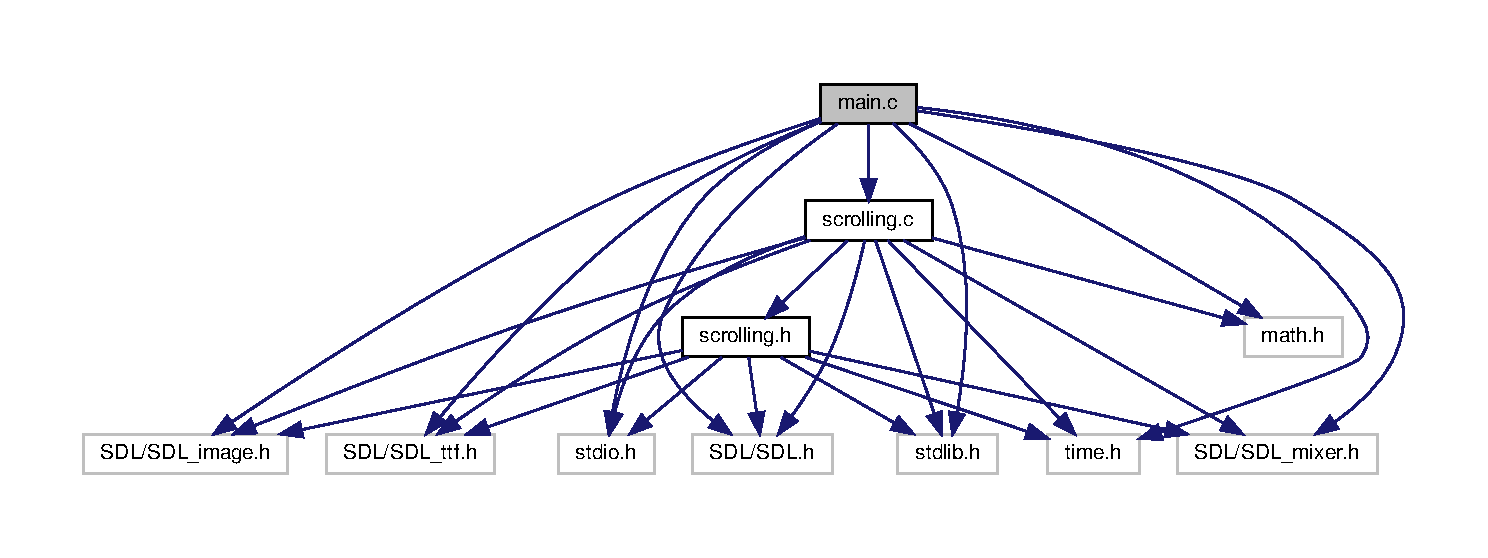
\includegraphics[width=350pt]{main_8c__incl}
\end{center}
\end{figure}
\subsection*{Functions}
\begin{DoxyCompactItemize}
\item 
int \hyperlink{main_8c_a0ddf1224851353fc92bfbff6f499fa97}{main} (int argc, char $\ast$argv\mbox{[}$\,$\mbox{]})
\end{DoxyCompactItemize}


\subsection{Function Documentation}
\mbox{\Hypertarget{main_8c_a0ddf1224851353fc92bfbff6f499fa97}\label{main_8c_a0ddf1224851353fc92bfbff6f499fa97}} 
\index{main.\+c@{main.\+c}!main@{main}}
\index{main@{main}!main.\+c@{main.\+c}}
\subsubsection{\texorpdfstring{main()}{main()}}
{\footnotesize\ttfamily int main (\begin{DoxyParamCaption}\item[{int}]{argc,  }\item[{char $\ast$}]{argv\mbox{[}$\,$\mbox{]} }\end{DoxyParamCaption})}

Here is the call graph for this function\+:\nopagebreak
\begin{figure}[H]
\begin{center}
\leavevmode
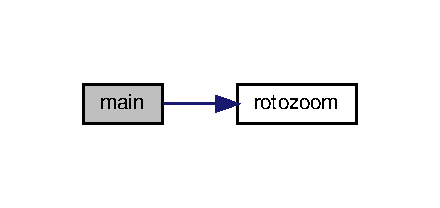
\includegraphics[width=211pt]{main_8c_a0ddf1224851353fc92bfbff6f499fa97_cgraph}
\end{center}
\end{figure}

\hypertarget{scrolling_8c}{}\section{scrolling.\+c File Reference}
\label{scrolling_8c}\index{scrolling.\+c@{scrolling.\+c}}
{\ttfamily \#include $<$stdlib.\+h$>$}\newline
{\ttfamily \#include $<$stdio.\+h$>$}\newline
{\ttfamily \#include $<$S\+D\+L/\+S\+D\+L\+\_\+image.\+h$>$}\newline
{\ttfamily \#include $<$S\+D\+L/\+S\+D\+L.\+h$>$}\newline
{\ttfamily \#include $<$S\+D\+L/\+S\+D\+L\+\_\+ttf.\+h$>$}\newline
{\ttfamily \#include $<$S\+D\+L/\+S\+D\+L\+\_\+mixer.\+h$>$}\newline
{\ttfamily \#include $<$time.\+h$>$}\newline
{\ttfamily \#include \char`\"{}scrolling.\+h\char`\"{}}\newline
{\ttfamily \#include $<$math.\+h$>$}\newline
Include dependency graph for scrolling.\+c\+:
\nopagebreak
\begin{figure}[H]
\begin{center}
\leavevmode
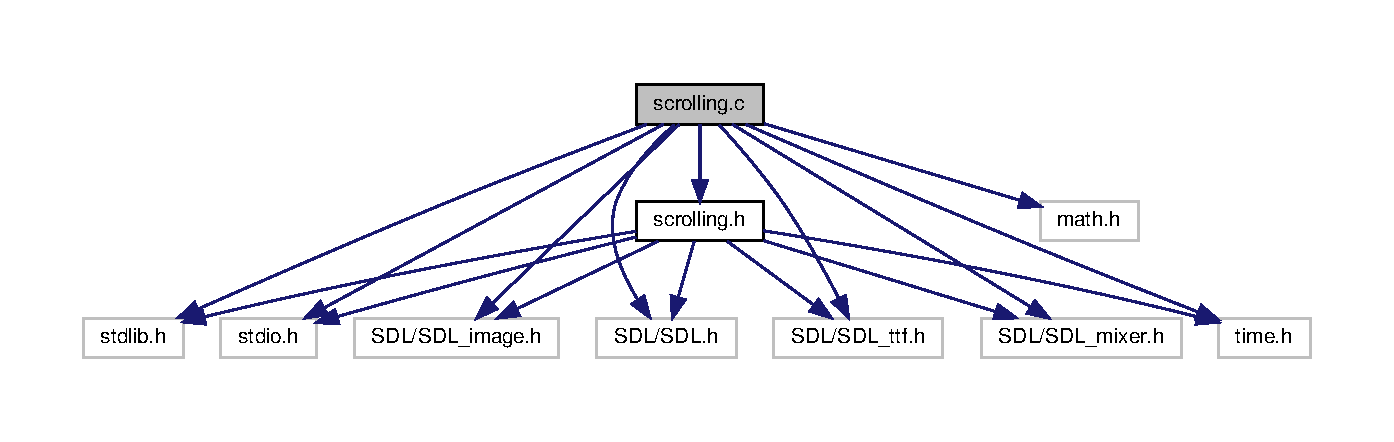
\includegraphics[width=350pt]{scrolling_8c__incl}
\end{center}
\end{figure}
This graph shows which files directly or indirectly include this file\+:
\nopagebreak
\begin{figure}[H]
\begin{center}
\leavevmode
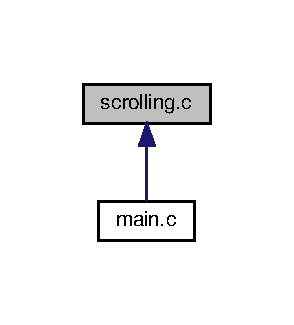
\includegraphics[width=141pt]{scrolling_8c__dep__incl}
\end{center}
\end{figure}
\subsection*{Functions}
\begin{DoxyCompactItemize}
\item 
void \hyperlink{scrolling_8c_adb8f7dc3d49f42765621f30ccc3d96db}{S\+C\+R\+O\+L\+L\+\_\+\+Init} (\hyperlink{structscrollImage}{scroll\+Image} $\ast$s, char $\ast$path)
\item 
void \hyperlink{scrolling_8c_ad1ec458216ea982b0e222f955f5b2002}{S\+C\+R\+O\+L\+L\+\_\+\+Render} (\hyperlink{structscrollImage}{scroll\+Image} $\ast$s, S\+D\+L\+\_\+\+Surface $\ast$$\ast$screen)
\item 
void \hyperlink{scrolling_8c_a4ca125812ab069b83f5692017d89e857}{animed} (S\+D\+L\+\_\+\+Rect animepos\mbox{[}$\,$\mbox{]}, int $\ast$frame)
\item 
void \hyperlink{scrolling_8c_a594ed7f200fc5f13125cbfab63bbad44}{animeg} (S\+D\+L\+\_\+\+Rect animepos\mbox{[}$\,$\mbox{]}, int $\ast$frame)
\item 
void \hyperlink{scrolling_8c_a2dafd7dbca163280e97acfd66e8d5780}{initialize\+Hero} (\hyperlink{structHero}{Hero} $\ast$hero)
\end{DoxyCompactItemize}


\subsection{Function Documentation}
\mbox{\Hypertarget{scrolling_8c_a4ca125812ab069b83f5692017d89e857}\label{scrolling_8c_a4ca125812ab069b83f5692017d89e857}} 
\index{scrolling.\+c@{scrolling.\+c}!animed@{animed}}
\index{animed@{animed}!scrolling.\+c@{scrolling.\+c}}
\subsubsection{\texorpdfstring{animed()}{animed()}}
{\footnotesize\ttfamily void animed (\begin{DoxyParamCaption}\item[{S\+D\+L\+\_\+\+Rect}]{animepos\mbox{[}$\,$\mbox{]},  }\item[{int $\ast$}]{frame }\end{DoxyParamCaption})}

Here is the caller graph for this function\+:
\nopagebreak
\begin{figure}[H]
\begin{center}
\leavevmode
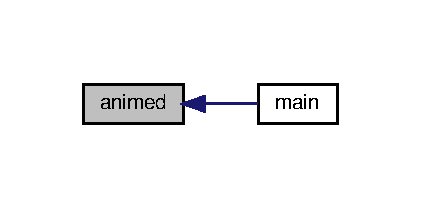
\includegraphics[width=202pt]{scrolling_8c_a4ca125812ab069b83f5692017d89e857_icgraph}
\end{center}
\end{figure}
\mbox{\Hypertarget{scrolling_8c_a594ed7f200fc5f13125cbfab63bbad44}\label{scrolling_8c_a594ed7f200fc5f13125cbfab63bbad44}} 
\index{scrolling.\+c@{scrolling.\+c}!animeg@{animeg}}
\index{animeg@{animeg}!scrolling.\+c@{scrolling.\+c}}
\subsubsection{\texorpdfstring{animeg()}{animeg()}}
{\footnotesize\ttfamily void animeg (\begin{DoxyParamCaption}\item[{S\+D\+L\+\_\+\+Rect}]{animepos\mbox{[}$\,$\mbox{]},  }\item[{int $\ast$}]{frame }\end{DoxyParamCaption})}

Here is the caller graph for this function\+:
\nopagebreak
\begin{figure}[H]
\begin{center}
\leavevmode
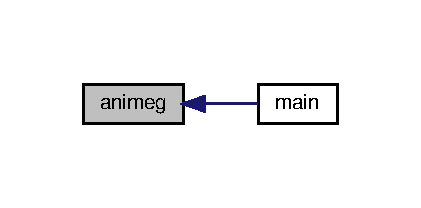
\includegraphics[width=202pt]{scrolling_8c_a594ed7f200fc5f13125cbfab63bbad44_icgraph}
\end{center}
\end{figure}
\mbox{\Hypertarget{scrolling_8c_a2dafd7dbca163280e97acfd66e8d5780}\label{scrolling_8c_a2dafd7dbca163280e97acfd66e8d5780}} 
\index{scrolling.\+c@{scrolling.\+c}!initialize\+Hero@{initialize\+Hero}}
\index{initialize\+Hero@{initialize\+Hero}!scrolling.\+c@{scrolling.\+c}}
\subsubsection{\texorpdfstring{initialize\+Hero()}{initializeHero()}}
{\footnotesize\ttfamily void initialize\+Hero (\begin{DoxyParamCaption}\item[{\hyperlink{structHero}{Hero} $\ast$}]{hero }\end{DoxyParamCaption})}

Here is the caller graph for this function\+:
\nopagebreak
\begin{figure}[H]
\begin{center}
\leavevmode
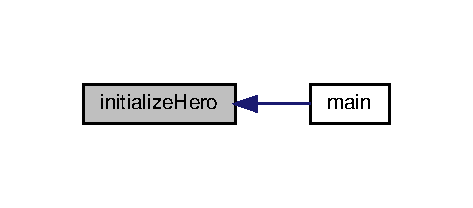
\includegraphics[width=227pt]{scrolling_8c_a2dafd7dbca163280e97acfd66e8d5780_icgraph}
\end{center}
\end{figure}
\mbox{\Hypertarget{scrolling_8c_adb8f7dc3d49f42765621f30ccc3d96db}\label{scrolling_8c_adb8f7dc3d49f42765621f30ccc3d96db}} 
\index{scrolling.\+c@{scrolling.\+c}!S\+C\+R\+O\+L\+L\+\_\+\+Init@{S\+C\+R\+O\+L\+L\+\_\+\+Init}}
\index{S\+C\+R\+O\+L\+L\+\_\+\+Init@{S\+C\+R\+O\+L\+L\+\_\+\+Init}!scrolling.\+c@{scrolling.\+c}}
\subsubsection{\texorpdfstring{S\+C\+R\+O\+L\+L\+\_\+\+Init()}{SCROLL\_Init()}}
{\footnotesize\ttfamily void S\+C\+R\+O\+L\+L\+\_\+\+Init (\begin{DoxyParamCaption}\item[{\hyperlink{structscrollImage}{scroll\+Image} $\ast$}]{s,  }\item[{char $\ast$}]{path }\end{DoxyParamCaption})}

Here is the caller graph for this function\+:
\nopagebreak
\begin{figure}[H]
\begin{center}
\leavevmode
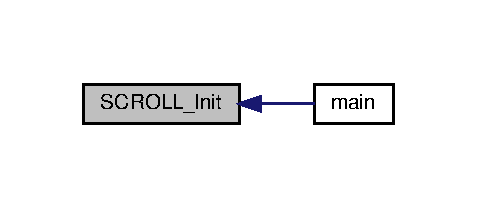
\includegraphics[width=229pt]{scrolling_8c_adb8f7dc3d49f42765621f30ccc3d96db_icgraph}
\end{center}
\end{figure}
\mbox{\Hypertarget{scrolling_8c_ad1ec458216ea982b0e222f955f5b2002}\label{scrolling_8c_ad1ec458216ea982b0e222f955f5b2002}} 
\index{scrolling.\+c@{scrolling.\+c}!S\+C\+R\+O\+L\+L\+\_\+\+Render@{S\+C\+R\+O\+L\+L\+\_\+\+Render}}
\index{S\+C\+R\+O\+L\+L\+\_\+\+Render@{S\+C\+R\+O\+L\+L\+\_\+\+Render}!scrolling.\+c@{scrolling.\+c}}
\subsubsection{\texorpdfstring{S\+C\+R\+O\+L\+L\+\_\+\+Render()}{SCROLL\_Render()}}
{\footnotesize\ttfamily void S\+C\+R\+O\+L\+L\+\_\+\+Render (\begin{DoxyParamCaption}\item[{\hyperlink{structscrollImage}{scroll\+Image} $\ast$}]{s,  }\item[{S\+D\+L\+\_\+\+Surface $\ast$$\ast$}]{screen }\end{DoxyParamCaption})}

Here is the caller graph for this function\+:
\nopagebreak
\begin{figure}[H]
\begin{center}
\leavevmode
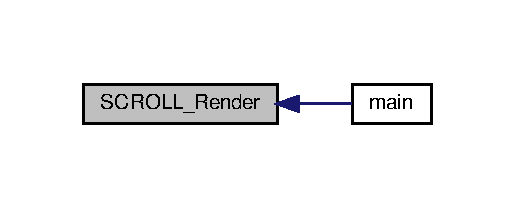
\includegraphics[width=247pt]{scrolling_8c_ad1ec458216ea982b0e222f955f5b2002_icgraph}
\end{center}
\end{figure}

\hypertarget{scrolling_8h}{}\section{scrolling.\+h File Reference}
\label{scrolling_8h}\index{scrolling.\+h@{scrolling.\+h}}
{\ttfamily \#include $<$stdlib.\+h$>$}\newline
{\ttfamily \#include $<$stdio.\+h$>$}\newline
{\ttfamily \#include $<$S\+D\+L/\+S\+D\+L\+\_\+image.\+h$>$}\newline
{\ttfamily \#include $<$S\+D\+L/\+S\+D\+L.\+h$>$}\newline
{\ttfamily \#include $<$S\+D\+L/\+S\+D\+L\+\_\+ttf.\+h$>$}\newline
{\ttfamily \#include $<$S\+D\+L/\+S\+D\+L\+\_\+mixer.\+h$>$}\newline
{\ttfamily \#include $<$time.\+h$>$}\newline
Include dependency graph for scrolling.\+h\+:
\nopagebreak
\begin{figure}[H]
\begin{center}
\leavevmode
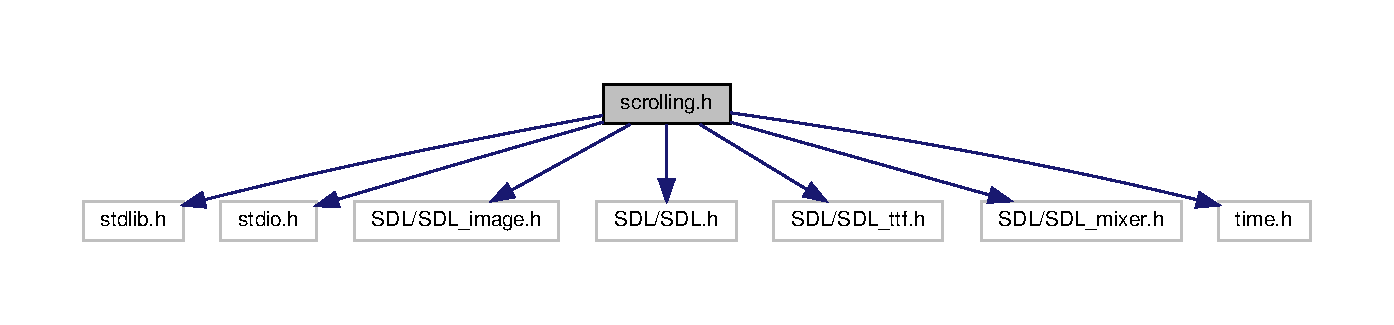
\includegraphics[width=350pt]{scrolling_8h__incl}
\end{center}
\end{figure}
This graph shows which files directly or indirectly include this file\+:
\nopagebreak
\begin{figure}[H]
\begin{center}
\leavevmode
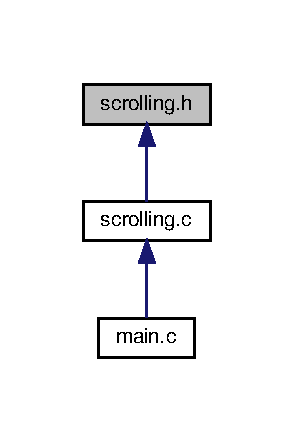
\includegraphics[width=141pt]{scrolling_8h__dep__incl}
\end{center}
\end{figure}
\subsection*{Classes}
\begin{DoxyCompactItemize}
\item 
struct \hyperlink{structHero}{Hero}
\item 
struct \hyperlink{structscrollImage}{scroll\+Image}
\end{DoxyCompactItemize}
\subsection*{Typedefs}
\begin{DoxyCompactItemize}
\item 
typedef struct \hyperlink{structHero}{Hero} \hyperlink{scrolling_8h_addc5c88d9738added14e95fd8f92b36f}{Hero}
\item 
typedef struct \hyperlink{structscrollImage}{scroll\+Image} \hyperlink{scrolling_8h_a0d83a8d1be6f5fe5d7281ce3b55cb875}{scroll\+Image}
\end{DoxyCompactItemize}
\subsection*{Functions}
\begin{DoxyCompactItemize}
\item 
void \hyperlink{scrolling_8h_adb8f7dc3d49f42765621f30ccc3d96db}{S\+C\+R\+O\+L\+L\+\_\+\+Init} (\hyperlink{structscrollImage}{scroll\+Image} $\ast$s, char $\ast$path)
\item 
void \hyperlink{scrolling_8h_ad1ec458216ea982b0e222f955f5b2002}{S\+C\+R\+O\+L\+L\+\_\+\+Render} (\hyperlink{structscrollImage}{scroll\+Image} $\ast$s, S\+D\+L\+\_\+\+Surface $\ast$$\ast$screen)
\item 
void \hyperlink{scrolling_8h_a2dafd7dbca163280e97acfd66e8d5780}{initialize\+Hero} (\hyperlink{structHero}{Hero} $\ast$hero)
\item 
void \hyperlink{scrolling_8h_a594ed7f200fc5f13125cbfab63bbad44}{animeg} (S\+D\+L\+\_\+\+Rect animepos\mbox{[}$\,$\mbox{]}, int $\ast$frame)
\item 
void \hyperlink{scrolling_8h_a4ca125812ab069b83f5692017d89e857}{animed} (S\+D\+L\+\_\+\+Rect animepos\mbox{[}$\,$\mbox{]}, int $\ast$frame)
\end{DoxyCompactItemize}
\subsection*{Variables}
\begin{DoxyCompactItemize}
\item 
double \hyperlink{scrolling_8h_af8ea4d2851d2d656fd42be239e36ce6e}{v\+\_\+x} = cos(\hyperlink{main_8c_ab8e20ab92095179ddfb4458f9c107090}{angle\+\_\+init})$\ast$\hyperlink{main_8c_ab16878bb20bd9d6028aa1300b223d3db}{v\+\_\+init}
\item 
double \hyperlink{scrolling_8h_a2161079bbf87834cfdf4d3548a53eb3b}{v\+\_\+y} = sin(\hyperlink{main_8c_ab8e20ab92095179ddfb4458f9c107090}{angle\+\_\+init})$\ast$\hyperlink{main_8c_ab16878bb20bd9d6028aa1300b223d3db}{v\+\_\+init}
\item 
const double \hyperlink{scrolling_8h_a6e550921d5c2c78c55be1c0d76512d45}{g} = 9.\+81
\item 
const double \hyperlink{scrolling_8h_a43016d873124d39034edb8cd164794db}{pi} = 3.\+14
\end{DoxyCompactItemize}


\subsection{Typedef Documentation}
\mbox{\Hypertarget{scrolling_8h_addc5c88d9738added14e95fd8f92b36f}\label{scrolling_8h_addc5c88d9738added14e95fd8f92b36f}} 
\index{scrolling.\+h@{scrolling.\+h}!Hero@{Hero}}
\index{Hero@{Hero}!scrolling.\+h@{scrolling.\+h}}
\subsubsection{\texorpdfstring{Hero}{Hero}}
{\footnotesize\ttfamily typedef struct \hyperlink{structHero}{Hero} \hyperlink{structHero}{Hero}}

\mbox{\Hypertarget{scrolling_8h_a0d83a8d1be6f5fe5d7281ce3b55cb875}\label{scrolling_8h_a0d83a8d1be6f5fe5d7281ce3b55cb875}} 
\index{scrolling.\+h@{scrolling.\+h}!scroll\+Image@{scroll\+Image}}
\index{scroll\+Image@{scroll\+Image}!scrolling.\+h@{scrolling.\+h}}
\subsubsection{\texorpdfstring{scroll\+Image}{scrollImage}}
{\footnotesize\ttfamily typedef struct \hyperlink{structscrollImage}{scroll\+Image}  \hyperlink{structscrollImage}{scroll\+Image}}



\subsection{Function Documentation}
\mbox{\Hypertarget{scrolling_8h_a4ca125812ab069b83f5692017d89e857}\label{scrolling_8h_a4ca125812ab069b83f5692017d89e857}} 
\index{scrolling.\+h@{scrolling.\+h}!animed@{animed}}
\index{animed@{animed}!scrolling.\+h@{scrolling.\+h}}
\subsubsection{\texorpdfstring{animed()}{animed()}}
{\footnotesize\ttfamily void animed (\begin{DoxyParamCaption}\item[{S\+D\+L\+\_\+\+Rect}]{animepos\mbox{[}$\,$\mbox{]},  }\item[{int $\ast$}]{frame }\end{DoxyParamCaption})}

Here is the caller graph for this function\+:
\nopagebreak
\begin{figure}[H]
\begin{center}
\leavevmode
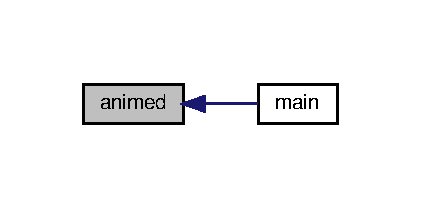
\includegraphics[width=202pt]{scrolling_8h_a4ca125812ab069b83f5692017d89e857_icgraph}
\end{center}
\end{figure}
\mbox{\Hypertarget{scrolling_8h_a594ed7f200fc5f13125cbfab63bbad44}\label{scrolling_8h_a594ed7f200fc5f13125cbfab63bbad44}} 
\index{scrolling.\+h@{scrolling.\+h}!animeg@{animeg}}
\index{animeg@{animeg}!scrolling.\+h@{scrolling.\+h}}
\subsubsection{\texorpdfstring{animeg()}{animeg()}}
{\footnotesize\ttfamily void animeg (\begin{DoxyParamCaption}\item[{S\+D\+L\+\_\+\+Rect}]{animepos\mbox{[}$\,$\mbox{]},  }\item[{int $\ast$}]{frame }\end{DoxyParamCaption})}

Here is the caller graph for this function\+:
\nopagebreak
\begin{figure}[H]
\begin{center}
\leavevmode
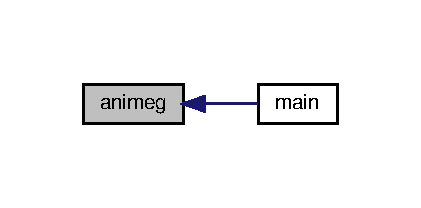
\includegraphics[width=202pt]{scrolling_8h_a594ed7f200fc5f13125cbfab63bbad44_icgraph}
\end{center}
\end{figure}
\mbox{\Hypertarget{scrolling_8h_a2dafd7dbca163280e97acfd66e8d5780}\label{scrolling_8h_a2dafd7dbca163280e97acfd66e8d5780}} 
\index{scrolling.\+h@{scrolling.\+h}!initialize\+Hero@{initialize\+Hero}}
\index{initialize\+Hero@{initialize\+Hero}!scrolling.\+h@{scrolling.\+h}}
\subsubsection{\texorpdfstring{initialize\+Hero()}{initializeHero()}}
{\footnotesize\ttfamily void initialize\+Hero (\begin{DoxyParamCaption}\item[{\hyperlink{structHero}{Hero} $\ast$}]{hero }\end{DoxyParamCaption})}

Here is the caller graph for this function\+:
\nopagebreak
\begin{figure}[H]
\begin{center}
\leavevmode
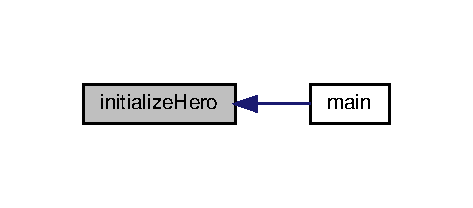
\includegraphics[width=227pt]{scrolling_8h_a2dafd7dbca163280e97acfd66e8d5780_icgraph}
\end{center}
\end{figure}
\mbox{\Hypertarget{scrolling_8h_adb8f7dc3d49f42765621f30ccc3d96db}\label{scrolling_8h_adb8f7dc3d49f42765621f30ccc3d96db}} 
\index{scrolling.\+h@{scrolling.\+h}!S\+C\+R\+O\+L\+L\+\_\+\+Init@{S\+C\+R\+O\+L\+L\+\_\+\+Init}}
\index{S\+C\+R\+O\+L\+L\+\_\+\+Init@{S\+C\+R\+O\+L\+L\+\_\+\+Init}!scrolling.\+h@{scrolling.\+h}}
\subsubsection{\texorpdfstring{S\+C\+R\+O\+L\+L\+\_\+\+Init()}{SCROLL\_Init()}}
{\footnotesize\ttfamily void S\+C\+R\+O\+L\+L\+\_\+\+Init (\begin{DoxyParamCaption}\item[{\hyperlink{structscrollImage}{scroll\+Image} $\ast$}]{s,  }\item[{char $\ast$}]{path }\end{DoxyParamCaption})}

Here is the caller graph for this function\+:
\nopagebreak
\begin{figure}[H]
\begin{center}
\leavevmode
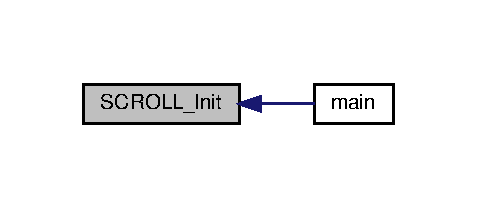
\includegraphics[width=229pt]{scrolling_8h_adb8f7dc3d49f42765621f30ccc3d96db_icgraph}
\end{center}
\end{figure}
\mbox{\Hypertarget{scrolling_8h_ad1ec458216ea982b0e222f955f5b2002}\label{scrolling_8h_ad1ec458216ea982b0e222f955f5b2002}} 
\index{scrolling.\+h@{scrolling.\+h}!S\+C\+R\+O\+L\+L\+\_\+\+Render@{S\+C\+R\+O\+L\+L\+\_\+\+Render}}
\index{S\+C\+R\+O\+L\+L\+\_\+\+Render@{S\+C\+R\+O\+L\+L\+\_\+\+Render}!scrolling.\+h@{scrolling.\+h}}
\subsubsection{\texorpdfstring{S\+C\+R\+O\+L\+L\+\_\+\+Render()}{SCROLL\_Render()}}
{\footnotesize\ttfamily void S\+C\+R\+O\+L\+L\+\_\+\+Render (\begin{DoxyParamCaption}\item[{\hyperlink{structscrollImage}{scroll\+Image} $\ast$}]{s,  }\item[{S\+D\+L\+\_\+\+Surface $\ast$$\ast$}]{screen }\end{DoxyParamCaption})}

Here is the caller graph for this function\+:
\nopagebreak
\begin{figure}[H]
\begin{center}
\leavevmode
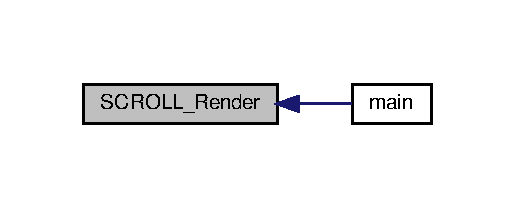
\includegraphics[width=247pt]{scrolling_8h_ad1ec458216ea982b0e222f955f5b2002_icgraph}
\end{center}
\end{figure}


\subsection{Variable Documentation}
\mbox{\Hypertarget{scrolling_8h_a6e550921d5c2c78c55be1c0d76512d45}\label{scrolling_8h_a6e550921d5c2c78c55be1c0d76512d45}} 
\index{scrolling.\+h@{scrolling.\+h}!g@{g}}
\index{g@{g}!scrolling.\+h@{scrolling.\+h}}
\subsubsection{\texorpdfstring{g}{g}}
{\footnotesize\ttfamily const double g = 9.\+81}

\mbox{\Hypertarget{scrolling_8h_a43016d873124d39034edb8cd164794db}\label{scrolling_8h_a43016d873124d39034edb8cd164794db}} 
\index{scrolling.\+h@{scrolling.\+h}!pi@{pi}}
\index{pi@{pi}!scrolling.\+h@{scrolling.\+h}}
\subsubsection{\texorpdfstring{pi}{pi}}
{\footnotesize\ttfamily const double pi = 3.\+14}

\mbox{\Hypertarget{scrolling_8h_af8ea4d2851d2d656fd42be239e36ce6e}\label{scrolling_8h_af8ea4d2851d2d656fd42be239e36ce6e}} 
\index{scrolling.\+h@{scrolling.\+h}!v\+\_\+x@{v\+\_\+x}}
\index{v\+\_\+x@{v\+\_\+x}!scrolling.\+h@{scrolling.\+h}}
\subsubsection{\texorpdfstring{v\+\_\+x}{v\_x}}
{\footnotesize\ttfamily double v\+\_\+x = cos(\hyperlink{main_8c_ab8e20ab92095179ddfb4458f9c107090}{angle\+\_\+init})$\ast$\hyperlink{main_8c_ab16878bb20bd9d6028aa1300b223d3db}{v\+\_\+init}}

\mbox{\Hypertarget{scrolling_8h_a2161079bbf87834cfdf4d3548a53eb3b}\label{scrolling_8h_a2161079bbf87834cfdf4d3548a53eb3b}} 
\index{scrolling.\+h@{scrolling.\+h}!v\+\_\+y@{v\+\_\+y}}
\index{v\+\_\+y@{v\+\_\+y}!scrolling.\+h@{scrolling.\+h}}
\subsubsection{\texorpdfstring{v\+\_\+y}{v\_y}}
{\footnotesize\ttfamily double v\+\_\+y = sin(\hyperlink{main_8c_ab8e20ab92095179ddfb4458f9c107090}{angle\+\_\+init})$\ast$\hyperlink{main_8c_ab16878bb20bd9d6028aa1300b223d3db}{v\+\_\+init}}


%--- End generated contents ---

% Index
\backmatter
\newpage
\phantomsection
\clearemptydoublepage
\addcontentsline{toc}{chapter}{Index}
\printindex

\end{document}
